%
% File acl-hlt2011.tex
%
% Contact: gdzhou@suda.edu.cn
%%
%% Based on the style files for ACL2008 by Joakim Nivre and Noah Smith
%% and that of ACL2010 by Jing-Shin Chang and Philipp Koehn


\documentclass[11pt]{article}
\usepackage{acl-hlt2011}
\usepackage{times}
\usepackage{latexsym}
\usepackage{amsmath}
\usepackage{multirow}
\usepackage{url}
\usepackage{float}
\usepackage{graphicx}

\DeclareMathOperator*{\argmax}{arg\,max}
\setlength\titlebox{6.5cm}    % Expanding the titlebox

\title{DLDE at 2014 Biomedical Summarization Track}

\author{Jie Chen \\
  Beijing Institute of Technology \\
  {\tt bit\_chenjie@bit.edu.cn} \\\And
  Zhendong Niu \\
  Beijing Institute of Technology \\
  {\tt zniu@bit.edu.cn} \\}

\date{}

\begin{document}
\maketitle
\begin{abstract}
In this note paper, we report our experiment method about task1a and task1b at biomedical summarization track 2014.

\end{abstract}



\section{System Overview}


\begin{figure}[H]
    \centering
    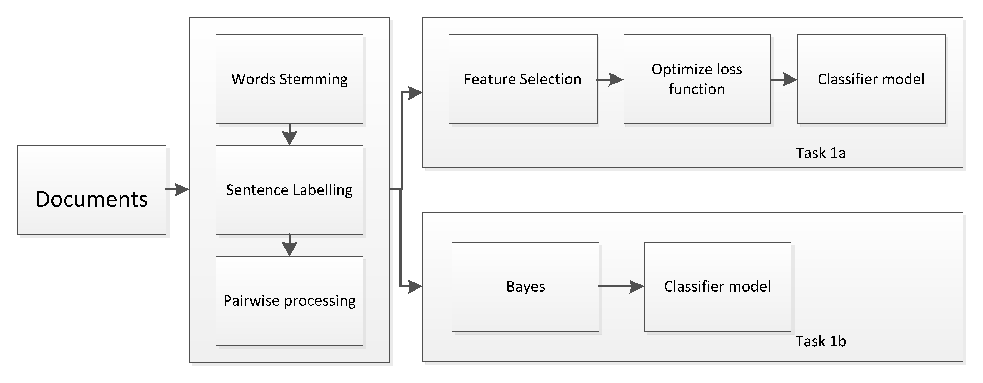
\includegraphics[height = 1.5in, width = 3.0in]{bio-frame2.eps}
    \caption{Overview of system framework}
    \label{fig:system-framework}
\end{figure}

Figure 1 outlines the structure of our system framework.
It can be devided into two parts.
One is prepared processing part which focus on word stemming, sentence labelling and pairwise processing.
The other one is model traning part which focus on training the classifier model for each task.



\section{Training data and processing}

{\bf Training Data in task1a}: Sentences are grouped into different pairs, each pair contains one sentence labeled in the RP and one sentence not labeled from the same RP paper.

{\bf Training Data in task1b}: Sentences that labeled as the most accurately reflect the citance in RP are selected with their facets to build the bayes classifier training data.


\section{Model}

{\bf Model in task1a}: 
First, We use the LSA to model the latent relationship among sentences in the same paper.
Second, the distance between the two sentences is computed.
Third, a loss function is introduced to measure the performance.
$$
Distance_{s_1,s_2} = \lambda_1x_{stat} + \lambda_2cosine(s_1,s_2)
$$
where $x_{stat}$ is the statistical feature subset of sentence bewteen $s_1, s_2$ such as the edit distance, the Jaccard distance.
$$
Loss = \sum_i^X(\sum^M_mDistance_{c_i, r_m} +\sum^N_n\frac{1}{Distance_{c_i, r_n}})
$$
where $c_i$ is the citance sentence in CP, $r_m$ is the labeled sentence in RP paper, $r_n$ is the sentence not labeled in RP paper.

{\bf Model in task1b}:In our opinion, the latent information about facet hide in some key words so that we choose the native bayes classifier to do this task.

$$
p(y|x) = \frac{p(x|y)p(y)}{p(x)}
$$
where $x$ is the word in the sentences and $y$ is defined by the labeled data.

\section{Results}

Three runs are submited for this task, the difference among them is the value selection about $\lambda1, \lambda2$ in the distance function.


\end{document}
